The calculation of electric fields is done by classes 
derived from the abstract base class \texttt{Component}. 
The key functions are 
\begin{lstlisting}
void ElectricField(const double x, const double y, const double z,
                   double& ex, double& ey, double& ez,
                   Medium*& m, int& status);
void ElectricField(const double x, const double y, const double z,
                   double& ex, double& ey, double& ez, double& v);
Medium* GetMedium(const double& x, const double& y, const double& z);
\end{lstlisting}
\begin{description}
  \item[x, y, z] 
  position where the electric field (medium) is to be determined
  \item[ex, ey, ez, v] 
  electric field and potential at the given position
  \item[m] pointer to the medium at the given position; 
  if there is no medium at this location, a null pointer is returned
  \item[status] status flag indicating where the point is located
  (see Table~\ref{Tab:StatusFlagsField})
\end{description}

\begin{table} 
  \centering
  \caption{Status flags for electric fields.}
  \label{Tab:StatusFlagsField}
  \begin{tabular}{l l}
  \toprule
  value & meaning \\
  \midrule
    0   & inside a drift medium \\
  \(> 0\) & inside a wire \\
   -1 \dots -4  &  on the side of a plane where no wires are \\
   -5   & inside the mesh, but not in a drift medium \\
   -6   & outside the mesh \\
  \bottomrule
  \end{tabular}
\end{table}

\section{Defining the geometry}

As mentioned above, the purpose of \texttt{Component} classes is to 
provide, for a given location, the electric (and magnetic) field and a pointer to the 
\texttt{Medium} object (if available).
For the latter task, it is obviously necessary to specify the geometry 
of the device. 
In case of field maps, the geometry is already defined in the field solver. 
It is, therefore, sufficient to associate the materials 
of the field map with the corresponding \texttt{Medium} objects. 

For analytic fields, the geometry is, in general, given by the 
cell layout.

For other components (\textit{e. g.} user-parameterized fields), 
the geometry has to be defined separately. 

Simple structures can be described by the native geometry (\texttt{GeometrySimple}), which has only a very restricted repertoire of shapes (solids). 
At present, the available solids are
\begin{itemize}
  \item
  \texttt{SolidBox}, 
  \item
  \texttt{SolidTube}, 
  \item
  \texttt{SolidHole}, 
  \item
  \texttt{SolidRidge},
  \item
  \texttt{SolidExtrusion}, 
  \item
  \texttt{SolidWire}, and
  \item
  \texttt{SolidSphere}.
\end{itemize} 
A description of these classes is given in Appendix \ref{Sec:Solids}.

As an example, we consider a gas-filled tube with a diameter of 1\,cm and 
a length of 20\,cm (along the \(z\)-axis), centred at the origin:
\begin{lstlisting}
// Create the medium.
MediumMagboltz gas;
// Create the geometry.
GeometrySimple geo;
// Dimensions of the tube
double rMax = 0.5, halfLength = 10.;
SolidTube tube(0., 0., 0., rMax, halfLength);
// Add the solid to the geometry, together with the gas inside.
geo.AddSolid(&tube, &gas);
\end{lstlisting}

Solids may overlap. 
When the geometry is scanned 
(triggered, for instance, by calling \texttt{GetMedium}), the  
first medium found is returned. 
The sequence of the scan is reversed with respect to the 
assembly of the geometry. 
Hence, the last medium added to the geometry is considered the innermost. 

For more complex structures, the class \texttt{GeometryRoot} can be used 
which provides an interface to the ROOT geometry (\texttt{TGeo}).
Using \texttt{GeometryRoot}, the above example would look like this:
\begin{lstlisting}
// Create the ROOT geometry.
TGeoManager* geoman = new TGeoManager("world", "geometry");
// Create the ROOT material and medium. 
// For simplicity we use the predefined material "Vacuum".
TGeoMaterial* matVacuum = new TGeoMaterial("Vacuum", 0, 0, 0);
TGeoMedium*   medVacuum = new TGeoMedium("Vacuum", 1, matVacuum);
// Dimensions of the tube
double rMin = 0., rMax = 0.5, halfLength = 10.;
// In this simple case, the tube is also the top volume.
TGeoVolume* top = geoman->MakeTube("TOP", medVacuum, rMin, rMax, halfLength);
geoman->SetTopVolume(top);
geoman->CloseGeometry();
// Create the Garfield medium.
MediumMagboltz* gas = new MediumMagboltz();
// Create the Garfield geometry.
GeometryRoot* geo = new GeometryRoot();
// Pass the pointer to the TGeoManager.
geo->SetGeometry(geoman);
// Associate the ROOT medium with the Garfield medium.
geo->SetMedium("Vacuum", gas); 
\end{lstlisting} 

In either case (\texttt{GeometrySimple} and \texttt{GeometryRoot}),
after assembly the geometry is passed to the \texttt{Component} as a pointer:
\begin{lstlisting}
void SetGeometry(Geometry* geo);
\end{lstlisting}

\subsection{Visualizing the geometry}

Geometries described by \texttt{GeometrySimple} can be viewed 
using the class \texttt{ViewGeometry}. 
\begin{lstlisting}
MediumMagboltz gas;
// Create and setup the geometry.
GeometrySimple geo;
const double r1 = 0.4;
const double r2 = 0.6;
SolidHole hole(0, 0, 0, r1, r2, 1, 1, 1);
hole.SetSectors(4);
geo.AddSolid(&hole, &gas);

// Create a viewer.
ViewGeometry geoView;
geoView.SetGeometry(&geo);
geoView.Plot3d();
\end{lstlisting}
The snippet above will produce a three-dimensional impression of the geometry.
The function \texttt{ViewGeometry::Plot2d()} draws a cut through the solids 
at the current viewing plane, \textit{e. g.} using again the geometry defined above,
\begin{lstlisting}
// ...
ViewGeometry geoView;
geoView.SetPlaneXZ();
geoView.Plot2d();
\end{lstlisting} 

%ROOT geometries can be visualized by calling the \texttt{Draw()} function of
%\texttt{TGeoManager}. 

The layout of an arrangement of wires, planes and tubes
defined in \texttt{ComponentAnalyticField} can be visualized using 
the member function
\begin{lstlisting}
void PlotCell(TPad* pad);
\end{lstlisting}
of \texttt{ComponentAnalyticField}:
\begin{lstlisting}
// Create and set up the component.
ComponentAnalyticField cmp;
// ...
TCanvas* canvas = new TCanvas("c", "", 600, 600);
cmp.PlotCell(canvas); 
\end{lstlisting}
This function internally uses the class \texttt{ViewCell}.
Instead of calling \texttt{PlotCell} one can also use \texttt{ViewCell} directly:
\begin{lstlisting}
// Create and set up the component.
ComponentAnalyticField cmp;
... 
// Create a viewer.
ViewCell view;
// Set the pointer to the component.
view.SetComponent(&cmp);
// Make a two-dimensional plot of the cell layout.
view.Plot2d();
\end{lstlisting}
By default, \texttt{ViewCell} will use marker symbols to indicate the position of the wires (instead of drawing the wires to scale). 
This behaviour can be switched on or off using the function
\begin{lstlisting}
ViewCell::EnableWireMarkers(const bool on);
\end{lstlisting} 
The function \texttt{ViewCell::Plot3d()} paints
a three-dimensional view of the cell layout.

\section{Field maps}

\subsection{Ansys}

\begin{figure}
\centering
\begin{tikzpicture}[line join=round,>=stealth]
\coordinate (n0) at ( 1.81,  4.31);
\coordinate (n1) at ( 1.00,  1.00);
\coordinate (n2) at ( 7.27,  1.00);
\coordinate (n3) at ( 8.35,  3.89);
\coordinate (n4) at ( 1.40,  2.66);
\coordinate (n5) at ( 4.13,  1.00);
\coordinate (n6) at ( 7.81,  2.45);
\coordinate (n7) at ( 5.08,  4.10);
\draw[thick,blue,->] (0,0) -- (9,0) node[below]{$x$};
\draw[thick,blue,->] (0,0) -- (0,5) node[left]{$y$};

\filldraw[black] (n0) circle (2pt) node[above left]{0};
\filldraw[black] (n1) circle (2pt) node[below left]{1};
\filldraw[black] (n2) circle (2pt) node[below right]{2};
\filldraw[black] (n3) circle (2pt) node[above right]{3};
\filldraw[black] (n4) circle (2pt) node[left]{4};
\filldraw[black] (n5) circle (2pt) node[below]{5};
\filldraw[black] (n6) circle (2pt) node[right]{6};
\filldraw[black] (n7) circle (2pt) node[above]{7};

\draw (n0) to[quadratic={(n4)}] (n1);
\draw (n1) to[quadratic={(n5)}] (n2);
\draw (n2) to[quadratic={(n6)}] (n3);
\draw (n3) to[quadratic={(n7)}] (n0);
\end{tikzpicture}
\caption{Eight-node quadrilateral element used in 2D Ansys field maps.}
\label{Fig:Plane121}
\end{figure}

\tdplotsetmaincoords{60}{120}
\begin{figure}
\centering
\begin{tikzpicture}[line join=round,>=stealth,tdplot_main_coords]
\coordinate (n0) at (-3.36, -1.40,  2.24);
\coordinate (n1) at ( 5.10, -0.94,  1.57);
\coordinate (n2) at (-4.36, -2.24, -4.56);
\coordinate (n3) at ( 0.61,  4.17,  0.75);
\coordinate (n4) at ( 0.87, -1.17,  1.90);
\coordinate (n5) at ( 0.37, -1.59, -1.49);
\coordinate (n6) at (-3.86, -1.82, -1.16);
\coordinate (n7) at (-1.37,  1.39,  1.49);
\coordinate (n8) at ( 2.86,  1.62,  1.16);
\coordinate (n9) at (-1.87,  0.97, -1.90);
\draw[thick,blue,->] (0,0,0) -- (5,0,0) node[below left]{$x$};
\draw[thick,blue,->] (0,0,0) -- (0,5,0) node[right]{$y$};
\draw[thick,blue,->] (0,0,0) -- (0,0,5) node[above]{$z$};

\filldraw[black] (n0) circle (2pt) node[above]{0};
\filldraw[black] (n1) circle (2pt) node[left]{1};
\filldraw[black] (n2) circle (2pt) node[below]{2};
\filldraw[black] (n3) circle (2pt) node[right]{3};
\filldraw[black] (n4) circle (2pt) node[above left]{4};
\filldraw[black] (n5) circle (2pt) node[below left]{5};
\filldraw[black] (n6) circle (2pt) node[right]{6};
\filldraw[black] (n7) circle (2pt) node[above right]{7};
\filldraw[black] (n8) circle (2pt) node[below]{8};
\filldraw[black] (n9) circle (2pt) node[below right]{9};

\draw (n0) to[quadratic={(n4)}] (n1);
\draw (n1) to[quadratic={(n5)}] (n2);
\draw (n2) to[quadratic={(n6)}] (n0);
\draw (n0) to[quadratic={(n7)}] (n3);
\draw[dashed] (n1) to[quadratic={(n8)}] (n3);
\draw (n2) to[quadratic={(n9)}] (n3);
\end{tikzpicture}
\caption{Ten-node tetrahedral element used in 3D Ansys field maps. The
         node numbering scheme shown here is the one used in Ansys 
         and differs slightly from the one used internally in 
         \texttt{ComponentAnsys123}.}
\label{Fig:Solid123}
\end{figure}

The interpolation of FEM field maps 
created with the program Ansys \cite{ANSYS} 
is dealt with by the classes
\texttt{ComponentAnsys121} and \texttt{ComponentAnsys123}. 
The class names refer to the type of mesh element used by Ansys:
\begin{itemize}
  \item
  \texttt{ComponentAnsys121} reads two-dimensional field maps 
  with eight-node curved quadrilaterals (Fig.~\ref{Fig:Plane121}),
  known as ``plane121'' in Ansys). 
  \item
  \texttt{ComponentAnsys123} reads three-dimensional field maps 
  with quadratic curved tetrahedra (Fig.~\ref{Fig:Solid123}),
  known as ``solid123'' in Ansys).
\end{itemize}

The field map is imported with the function
\begin{lstlisting}
bool Initialise(std::string elist, std::string nlist,
                std::string mplist, std::string prnsol, std::string unit);
\end{lstlisting}
\begin{description}
  \item[elist]
  name of the file containing the list of elements 
  (default: \texttt{"ELIST.lis"})
  \item[nlist]
  name of the file containing the list of nodes
  (default: \texttt{"NLIST.lis"})
  \item[mplist]
  name of the file containing the list of materials
  (default: \texttt{"MPLIST.lis"})
  \item[prnsol]
  name of the file containing the nodal solutions
  (default: \texttt{"PRNSOL.lis"})
  \item[unit]
  length unit used in the calculation (default: \texttt{"cm"}, \\ 
  other recognized units are 
  \texttt{"mum"}/\texttt{"micron"}/\texttt{"micrometer"},
  \texttt{"mm"}/\texttt{"millimeter"} and 
  \texttt{"m"}/\texttt{"meter"}).
\end{description}
The return value is \texttt{true} if the map was read successfully.

In order to enable charge transport and ionization,
the materials in the map need to be associated with \texttt{Medium} objects.
\begin{lstlisting}
// Get the number of materials in the map.
size_t GetNumberOfMaterials();
// Associate a material with a Medium object.
void SetMedium(const size_t imat, Medium* medium);
\end{lstlisting}
\begin{description}
\item[imat]
index in the list of (field map) materials
\item[medium]
pointer to the \texttt{Medium} object to be associated with this material
\end{description}

The materials in the field map are characterized by the 
relative dielectric constant \(\varepsilon\) and the 
conductivity \(\sigma\). 
These parameters are accessible through the functions
\begin{lstlisting}
double GetPermittivity(const size_t imat);
double GetConductivity(const size_t imat);
\end{lstlisting}
The function
\begin{lstlisting}
void SetGas(Medium* medium);
\end{lstlisting}
associates a given \texttt{Medium} object to all field map materials 
with $\varepsilon = 1$.
 
By default, mesh elements in conductors, \ie materials 
with resistivity equal to zero, are eliminated. This feature can be 
switched on or off using
\begin{lstlisting}
void EnableDeleteBackgroundElements(const bool on = true);
\end{lstlisting}
\begin{description}
  \item[on] flag to delete mesh elements in conductors (\texttt{true}) or keep them (\texttt{false}) 
\end{description}
A weighting field map can be imported using
\begin{lstlisting}
bool SetWeightingField(std::string prnsol, std::string label);
\end{lstlisting}
\begin{description}
  \item[prnsol]
  name of the file containing the nodal solution for the weighting field
  configuration
  \item[label]
  arbitrary name, used for identification of the electrode/signal
\end{description}

The weighting field map has to use the same mesh as the previously 
read ``actual'' field map.

For periodic structures, \textit{e.\,g.} GEMs, one usually models only 
the basic cell of the geometry and applies appropriate symmetry 
conditions to cover the whole problem domain. 
The available symmetry operations are:
\begin{itemize}
  \item
  simple periodicities,
  \item
  mirror periodicities, 
  \item
  axial periodicities, and
  \item
  rotation symmetries.
\end{itemize}

Mirror periodicity means that odd periodic copies of the basic cell 
are mirror images of even periodic copies.
Mirror periodicity and simple periodicity as well as 
axial periodicity and rotation symmetry are, 
obviously, mutually exclusive. 
In case of axial periodicity, the field map has to cover an 
integral fraction of \(2\pi\). 

Periodicities can be set and unset using
\begin{lstlisting}
void EnablePeriodicityX(const bool on);
void EnableMirrorPeriodicityX(const bool on);
void EnableAxialPeriodicityX(const bool on);
void EnableRotationSymmetryX(const bool on);
\end{lstlisting}
\begin{description}
\item[on] flag to enable (\texttt{true}) or disable (\texttt{false}) periodicity. 
\end{description}
Analogous functions are available for \(y\) and \(z\).

In order to assess the quality of the mesh, 
one can retrieve the dimensions of each mesh element using
\begin{lstlisting}
bool GetElement(const size_t i, double& vol, double& dmin, double& dmax);
\end{lstlisting}
\begin{description}
\item[i] index of the element
\item[vol] volume/area of the element
\item[dmin, dmax] min./max. distance between two node points
\end{description}

In the following example we make histograms of the aspect ratio and 
element size.
\begin{lstlisting}
ComponentAnsys123* fm = new ComponentAnsys123();
...
TH1F* hAspectRatio = new TH1F("hAspectRatio"; "Aspect Ratio", 100, 0., 50.);
TH1F* hSize = new TH1F("hSize", "Element Size", 100, 0., 30.);
const size_t nel = fm->GetNumberOfElements();
// Loop over the elements.
double volume, dmin, dmax;
for (size_t i = 0; i < nel; ++i) {
  fm->GetElement(i, volume, dmin, dmax);
  if (dmin > 0.) hAspectRatio->Fill(dmax / dmin);
  hSize->Fill(volume);
}
TCanvas* c1 = new TCanvas();
hAspectRatio->Draw();
TCanvas* c2 = new TCanvas();
c2->SetLogy();
hSize->Draw();
\end{lstlisting}

Since Ansys uses curved elements, an iterative procedure is used for 
determining the local coordinates of a point within an element. 
This search can sometimes fail to achieve the requested precision.
In this case, the first-order approximation is used, and (by default) 
a warning message is printed out. These messages can be switched on or off 
using 
\begin{lstlisting}
void EnableConvergenceWarnings(const bool on);
\end{lstlisting}

\subsection{Synopsys TCAD}

Electric fields calculated using the device simulation program 
Synopsys Sentaurus \cite{Synopsys} can be imported with the classes 
\texttt{ComponentTcad2d} and \texttt{ComponentTcad3d} (derived from 
the base class \texttt{ComponentTcadBase}).

The function to import the field map is 
\begin{lstlisting}
bool Initialise(const std::string& gridfilename,
                const std::string& datafilename);
\end{lstlisting}
\begin{description}
  \item[gridfilename]
  name of the mesh file, the extension is typically \texttt{.grd}
  \item[datafilename]
  name of the file containing the nodal solution;
  the filename typically typically ends with \texttt{\_des.dat}
\end{description}

Both files have to be exported in DF-ISE format, 
files in the default TDR format cannot be read.
To convert a TDR file to \texttt{\_.dat} and \texttt{.grd} files, the
Sentaurus tool \texttt{tdx} can be used
\begin{lstlisting}
tdx -dd fieldToConvert.tdr
\end{lstlisting}

The classes have been tested with meshes created with the application 
\texttt{Mesh} which can produce axis-aligned 
two- and three-dimensional meshes.
The only three-dimensional mesh elements \texttt{ComponentTcad3d} 
can deal with are tetrahedra. 
A mesh which consists only of simplex elements 
(triangles in 2D, tetrahedra in 3D), 
can be generated by invoking \texttt{Mesh} with the option \texttt{-t}.

After importing the files, 
the regions of the device where charge transport is to be enabled 
need to be associated with \texttt{Medium} objects. 
\begin{lstlisting}
// Get the number of regions in the device
size_t GetNumberOfRegions();
// Associate a region with a Medium object 
void SetMedium(const size_t ireg, Medium* medium);
\end{lstlisting}
\begin{description}
  \item[ireg]
  index in the list of device regions
  \item[medium]
  pointer to the \texttt{Medium} object to be associated with this region
\end{description}
To associate all regions with certain material to a given \texttt{Medium} 
object, one can use the function
\begin{lstlisting}
void SetMedium(const std::string& material, Medium* medium);
\end{lstlisting}
\begin{description}
  \item[material] name of the material in TCAD
  \item[medium] pointer to the \texttt{Medium} to be associated to all regions with this material.
\end{description}

The name of a region can be retrieved with
\begin{lstlisting}
void GetRegion(const size_t i, std::string& name, bool& active);
\end{lstlisting}
\begin{description}
  \item[name] 
  label of the region as defined in the device simulation
  \item[active] 
  flag indicating whether charge transport is enabled 
  in this region
\end{description}

Simple periodicities and mirror periodicities along 
\(x\), \(y\), and -- in case of \texttt{ComponentTcad3d} -- \(z\) 
are supported. 
\begin{lstlisting}
void EnablePeriodicityX();
void EnableMirrorPeriodicityX();
\end{lstlisting}

Using TCAD, the weighting field and potential are typically determined 
by first computing the electric field $\mathbf{E}_{0}$ and potential 
$V_{0}$ with all electrodes set at the nominal potentials.
The potential at the electrode to be read out is then increased by a 
small voltage $\Delta V$ and the corresponding electric field $E_{+}$ and 
potential $V_{+}$ are calculated. The weighting field and potential 
are then given by 
\begin{equation*}
  \mathbf{E}_{w} = \frac{1}{\Delta V}\left(\mathbf{E}_{+} - \mathbf{E}_{0}\right), \qquad V_{w} = \frac{1}{\Delta V}\left(V_{+} - V_{0}\right).
\end{equation*}
In \texttt{ComponentTcad2d} and \texttt{ComponentTcad3d} the weighting 
field and potential loaded using
\begin{lstlisting} 
SetWeightingField(const std::string& datfile1, const std::string& datfile2,
                  const double dv, const std::string& label); 
\end{lstlisting}
\begin{description}
  \item[datfile1] \texttt{.dat} file containing the solution $\mathbf{E}_0, V_0$,
  \item[datfile2] \texttt{.dat} file containing the solution $\mathbf{E}_+, V_+$,
  \item[dv] potential difference $\Delta V$,
  \item[label] identifier of the electrode.
\end{description}
The mesh is assumed to be the same as the one for the drift field 
(imported using \texttt{Initialise}).

Using the function
\begin{lstlisting}
bool SetWeightingFieldShift(const std::string& label,
                            const double x, const double y, const double z);
\end{lstlisting}
one can set an offset to be applied to the map of weighting fields and potentials imported from TCAD.

\subsection{Elmer}

The class \texttt{ComponentElmer} (contributed by J. Renner) allows one to import 
field maps created with the open source field solver Elmer \cite{Elmer}
and the mesh tool Gmsh \cite{Gmsh}. 
A detailed tutorial can be found on the webpage. 

\subsection{CST}

The class \texttt{ComponentCST} (contributed by K.~Zenker) reads field maps 
extracted from CST Studio. More details can be found at 
\href{http://www.desy.de/~zenker/FLC/garfieldpp.html}{http://www.desy.de/~zenker/FLC/garfieldpp.html}.

\subsection{COMSOL}

The class \texttt{ComponentComsol} (contributed by E.~Bodnia) can be used for 
importing field maps computed using COMSOL Multiphysics.
The function to import a field map is 
\begin{lstlisting}
bool Initialise(std::string header = "mesh.mphtxt",
                std::string mplist = "dielectrics.dat",
                std::string field = "field.txt");
\end{lstlisting}
\begin{description}
  \item[header] COMSOL Multiphysics text file (\texttt{.mphtxt}) containing the mesh data,
  \item[mplist] file containing the material properties, 
  \item[field] file containing the exported field data. 
\end{description}
The materials file (second argument) is a simply ASCII file containing
\begin{itemize}
  \item
  the number of materials in the field map, 
  \item
  the relative dielectric constants of each of the materials,
  \item
  the number of ``domains'',
  \item
  a list of domain numbers and indices of the corresponding materials.
\end{itemize}
The domain numbers can be found in the section 
\texttt{\# Geometric entity indices} of the mesh data file 
(\texttt{mesh.mphtxt}).
For a field map with two materials, 
one with a dielectric constant of $\varepsilon = 1$ (domain number 1) and 
the other one with a dielectric constant of $\varepsilon = 4$ 
(domain number 2), the file should look like the following.
\begin{lstlisting}
2
1. 4. 
2
1 0
2 1
\end{lstlisting}

\subsection{Regular grids}
\begin{figure}
  \centering
  \begin{tikzpicture}
    \draw[help lines,step=2] (0, 0) grid (6, 4);
    \foreach \x in {0,2,4,6}
    \foreach \y in {0,2,4} {
      \fill (\x,\y) circle (2pt);
    }
    \node[below] at (0,0) {\footnotesize $x_{\text{min}}$};
    \node[below] at (6,0) {\footnotesize $x_{\text{max}}$};
    \node[left] at (0,0) {\footnotesize $y_{\text{min}}$};
    \node[left] at (0,4) {\footnotesize $y_{\text{max}}$};
    \node[above right] at (0,0) {\footnotesize $\left(0,0\right)$};
    \node[above right] at (6,0) {\footnotesize $\left(3,0\right)$};
    \node[above right] at (6,4) {\footnotesize $\left(3,2\right)$};
  \end{tikzpicture}
  \caption{Example of a two-dimensional regular mesh (as used in 
           \texttt{ComponentGrid}) with $4\times3$ grid points, 
           corresponding to $n_{x} = 4, n_{y} = 3$.} 
  \label{Fig:MeshComponentGrid}
\end{figure}
Electric field values on a regular two-dimensional or three-dimensional grid 
can be imported from a text file using the class \texttt{ComponentGrid}. 
The electric field values (and potential) for each point on the grid 
are read in using
\begin{lstlisting}
bool LoadElectricField(const std::string& filename, const std::string& format,
                       const bool withPotential, const bool withFlag,
                       const double scaleX = 1., const double scaleE = 1.,
                       const double scaleP = 1.);
\end{lstlisting}
\begin{description}
  \item[filename]
  name of the ASCII file
  \item[format]
  description of the file format (see below)
  \item[withPotential]
  flag whether the file contains an additional column with the electrostatic potential
  \item[withRegion]
  flag whether the file contains an additional column with an integer value 
  indicating whether the point is in an active medium (1) or not (0).
  \item[scaleX, scaleE, scaleP]
  scaling factors to be applied to the coordinates, electric field values 
  and potentials 
\end{description}
The file should contain one line for each grid point.
The available formats are \texttt{XY}, \texttt{XZ}, \texttt{IJ}, 
\texttt{IK}, \texttt{XYZ} and \texttt{IJK}, the first four 
for two-dimensional maps, and the 
last two for three-dimensional maps.
In case of \texttt{XY} (\texttt{XYZ}), the first two (three) columns  
contain the $x$, $y$ (and $z$) coordinates of a given point in the 
grid, followed by the electric field values (and potential if available) at 
this point. The class then determines the closest grid point 
and assigns the electric field and potential accordingly.
In case of \texttt{IJ} (\texttt{IJK}) the indices of the grid point 
along $x$, $y$ (and $z$) are specified directly.
The file can include comments (lines starting with \texttt{\#} or \texttt{//}). 

Prior to reading the electric field, the limits and spacing of the grid 
can be set using the function
\begin{lstlisting}
void SetMesh(const unsigned int nx, const unsigned int ny,
             const unsigned int nz, const double xmin, const double xmax,
             const double ymin, const double ymax, const double zmin,
             const double zmax);
\end{lstlisting}
\begin{description}
  \item[nx, ny, nz] 
  number of grid lines along $x$, $y$, $z$
  \item[xmin, xmax, \dots] 
  boundaries of the grid in $x$, $y$, $z$
\end{description}
An example illustrating the parameters defining the mesh and the 
numbering of the grid nodes is shown in Fig.~\ref{Fig:MeshComponentGrid}.
Alternatively, the grid parameters can be read from the file that contains
the electric field/potential. For instance, to specify the 
limits and number of grid lines along $z$, a line like 
\begin{lstlisting}
# ZMIN = -1., ZMAX = 1., NZ = 3 
\end{lstlisting} 
should be included at the beginning of the file.
If the user has not specified the grid explicitly (using \texttt{SetMesh}) 
and the information given in the comment lines is incomplete, the 
class will try to determine the remaining grid parameters from the 
table of coordinates and corresponding electric fields itself.

When retrieving the field/potential at a given point $\left(x, y, z\right)$ 
the class performs a trilinear interpolation between the values at the 
grid nodes surrounding this point. The medium in the domain covered by the mesh 
is set using 
\begin{lstlisting}
void SetMedium(Medium* m);
\end{lstlisting}
A point $\left(x,y,z\right)$ is considered in an active region 
(\ie associated to the medium) if all surrounding grid nodes are 
flagged as active. 

A magnetic field map can be imported using the function
\begin{lstlisting}
bool LoadMagneticField(const std::string& filename, const std::string& format,
                       const double scaleX = 1., const double scaleB = 1.);
\end{lstlisting}
The available formats are the same as for the electric field (except for the 
extra columns for potential and active medium flag).
Prompt and delayed weighting fields/potentials can be imported using
\begin{lstlisting}
bool LoadWeightingField(const std::string& filename, const std::string& format,
                        const bool withPotential,
                        const double scaleX = 1., const double scaleE = 1.,
                        const double scaleP = 1.);
bool LoadWeightingField(const std::string& filename, const std::string& format,
                        const double time, const bool withPotential,
                        const double scaleX = 1., const double scaleE = 1.,
                        const double scaleP = 1.);
\end{lstlisting}

Calling 
\begin{lstlisting}
void SetCylindricalCoordinates();
\end{lstlisting}
switches to a cylindrical coordinate system instead of the default Cartesian coordinates.
The first coordinate ("x") then corresponds to the radial distance 
and the second coordinate ("y") corresponds to the azimuth (in radian).

\begin{figure}
  \centering
  \begin{tikzpicture}
    \draw[help lines,step=2] (0, 0) grid (6, 4);
    \foreach \x in {1,3,5}
    \foreach \y in {1,3} {
      \fill (\x,\y) circle (2pt);
    }
    \node[below] at (0,0) {\footnotesize $x_{\text{min}}$};
    \node[below] at (6,0) {\footnotesize $x_{\text{max}}$};
    \node[left] at (0,0) {\footnotesize $y_{\text{min}}$};
    \node[left] at (0,4) {\footnotesize $y_{\text{max}}$};
    \node[above right] at (1,1) {\footnotesize $\left(0,0\right)$};
    \node[above right] at (5,1) {\footnotesize $\left(2,0\right)$};
    \node[above right] at (5,3) {\footnotesize $\left(2,1\right)$};
  \end{tikzpicture}
  \caption{Example of a two-dimensional regular mesh (as used in 
           \texttt{ComponentVoxel}) with $3\times2$ cells, 
           corresponding to $n_{x} = 3, n_{y} = 2$.} 
  \label{Fig:MeshComponentVoxel}
\end{figure}

The class \texttt{ComponentVoxel} is similar to \texttt{ComponentGrid} 
but uses a different definition of the mesh. 
An example illustrating the parameters of the mesh and the numbering of 
the voxels/cells is shown in Fig.~\ref{Fig:MeshComponentVoxel}.
As a first step, the mesh needs to be defined using the function
\begin{lstlisting}
void SetMesh(const unsigned int nx, const unsigned int ny,
             const unsigned int nz, const double xmin, const double xmax,
             const double ymin, const double ymax, const double zmin,
             const double zmax);
\end{lstlisting}
\begin{description}
  \item[nx, ny, nz] 
  number of rows/columns of cells along $x$, $y$, $z$
  \item[xmin, xmax, \dots] 
  boundaries of the grid in $x$, $y$, $z$
\end{description}
The electric field values (and potential) for each voxel are imported using 
\begin{lstlisting}
bool LoadElectricField(const std::string& filename, const std::string& format,
                       const bool withPotential, const bool withRegion,
                       const double scaleX = 1., const double scaleE = 1.,
                       const double scaleP = 1.);
\end{lstlisting}
\begin{description}
  \item[filename]
  name of the ASCII file
  \item[format]
  description of the file format (see \texttt{ComponentGrid})
  \item[withPotential]
  flag whether the file contains an additional column with the electrostatic potential
  \item[withRegion]
  flag whether the file contains an additional column with an integer value 
  corresponding to the region index (each region can be associated with a different medium)
  \item[scaleX, scaleE, scaleP]
  scaling factors to be applied to the coordinates, electric field values 
  and potentials 
\end{description}
The medium to be associated with a given region can be set using
\begin{lstlisting}
void SetMedium(const unsigned int i, Medium* m);
\end{lstlisting}
\begin{description}
  \item[i] index of the region
\end{description}
If the regions are not assigned explicitly when importing the electric field, 
all voxels are assumed to belong to the same region (index 0).

By default, the field and potential are assumed to be constant within 
a voxel. Alternatively, the fields/potentials given in the field map file
can be interpreted to be the values at the voxel centres and the 
fields/potentials at intermediate points be determined by trilinear interpolation.
This feature can be activated using the function
\begin{lstlisting}
void EnableInterpolation(const bool on = true);
\end{lstlisting} 
 
\subsection{Visualizing the mesh}

For visualizing the mesh imported from a FEM field map, the class 
\texttt{ViewFEMesh} (written by J. Renner) is available. 
Using 
\begin{lstlisting}
void ViewFEMesh::SetViewDrift(ViewDrift* driftView);
\end{lstlisting}
a \texttt{ViewDrift} object can be attached to the mesh viewer. 
The function
\begin{lstlisting}
bool ViewFEMesh::Plot();
\end{lstlisting}
then allows draws a two-dimensional projection of the drift lines stored in the  
\texttt{ViewDrift} class together with the mesh. 
The plot can be customized using 
\begin{lstlisting}
void SetColor(int matid, int colorid);
void SetFillColor(int matid, int colorid);
void SetFillMesh(bool fill);
\end{lstlisting}
\begin{description}
  \item[matid] material index in the field map
  \item[colorid] index of the ROOT color with which all elements of material 
                 \texttt{matid} are to be drawn 
  \item[fill] flag indicating whether to draw a wireframe mesh (\texttt{false}) 
              or filled elements
\end{description}
As an illustration consider the following example 
(suppose that \texttt{fm} is a pointer to a field map component 
and \texttt{driftView} is a pointer to a \texttt{ViewDrift} object) 
\begin{lstlisting}
  TCanvas* c1 = new TCanvas();
  ViewFEMesh* meshView = new ViewFEMesh();
  meshView->SetCanvas(c1);
  // Set the component.
  meshView->SetComponent(fm);
  // Set the viewing plane.
  meshView->SetPlane(0, -1, 0, 0, 0, 0);
  meshView->SetFillMesh(false);
  meshView->SetViewDrift(driftView);
  meshView->SetArea(-0.01, -0.01, -0.03, 0.01, 0.01, 0.01);
  meshView->Plot();
\end{lstlisting}

\section{Analytic fields}

For two-dimensional geometries consisting of wires, planes and tubes, 
semi-analytic calculation techniques are implemented. 
The equations to be solved to find the wire charges are known as 
capacitance equations, they are obtained by expressing the (known) 
potential of wire $i$ in the (unknown) charges per unit length $q_j$ 
on the wires $j = 1 \dots n$,
\begin{equation*}
V_{i} = \sum\limits_{j=1}^{n} C_{ij}^{-1}q_{j} + V_{\text{ref}} 
\end{equation*}
When planes are absent, the freedom to choose a reference potential 
$V_{\text{ref}}$ can be exploited to ensure that the sum of all 
charges is zero, by adding 
\begin{equation*}
\sum\limits_{j=1}^{n} q_{j} = 0
\end{equation*}
to the set of equations.
If there is at least one equipotential plane, the sum of all charges 
is automatically zero (the charges and mirror charges cancel) and 
the reference potential is set equal to zero in this case.

The equipotential planes can be treated as if they were grounded 
if the linear potential generated by the planes alone is subtracted 
from all wire-potentials before the charges are calculated and 
added separately when the potential and electrostatic field are evaluated.

\subsection{Describing the cell}
The medium to be associated with the active region of the cell 
is set using
\begin{lstlisting}
SetMedium(Medium* medium);
\end{lstlisting}
Wires, tubes and planes can be added to the cell layout by means of the 
following functions:
\begin{lstlisting}
// Add a wire
void AddWire(const double x, const double y, const double d,
             const double v, const std::string& label = "", 
             const double length = 100.,
             const double tension = 50., const double rho = 19.3);
// Add a tube
void AddTube(const double r, const double v, 
             const int nEdges, const std::string& label = "");
// Add a plane at constant x
void AddPlaneX(const double x, const double v, const std::string& label = "");
// Add a plane at constant y
void AddPlaneY(const double y, const double v, const std::string& label = "");
\end{lstlisting} 

All of these functions take the potential \texttt{v} (in V) 
and a label as arguments. 
The \texttt{label} argument is optional. If the default value 
(empty string) is used, the calculation of the weighting field and potential for this wire, tube or plane will be skipped (\textit{i. e.} one cannot compute the signal induced in this element).
 
For wires, the center of the wire (\texttt{x, y}) 
and its diameter (\texttt{d}) need to be specified. 
Optional parameters are the wire length, the tension (more precisely, the 
mass in g of the weight used to stretch the wire during the assembly) and 
the density (in g\,/\,cm\(^{3}\)) of the wire material. 
These parameters have no influence on the electric field. 
The number of wires that can be added is not limited.

Tube-specific parameters are the radius\footnote{For non-circular tubes, this parameter is the distance between the origin and any of the edges.} (\texttt{r}) and the number of edges, which determines the shape of the tube:
  \begin{itemize}
    \item
    \(n = 0\): cylindrical pipe
    \item
    \(3 \le n \le 8\): regular polygon 
  \end{itemize}
There can be only one tube in a cell. 
The tube is always centered at the origin \(\left(0, 0\right)\).

Planes are described by their coordinates. 
A cell can have at most two \(x\) and two \(y\) planes. 
Planes and tubes cannot be used together in the same cell.

The geometry can be reset (thereby deleting all wires, planes and tubes) by
\begin{lstlisting}
void Clear();
\end{lstlisting}

Before assembling and inverting the capacitance matrix, 
a check is performed whether the provided geometry matches the requirements.
If necessary, the planes and wires are reordered. 
Wires outside the tube or the planes as well as overlapping wires are removed.

\subsection{Cylindrical geometries}

By default, the wire coordinates are specified in Cartesian coordinates and 
the planes are parallel to the $x$ or $y$ axis.
Calling 
\begin{lstlisting}
void SetPolarCoordinates();
\end{lstlisting} 
switches to a polar coordinate system. This can be useful for 
certain types of cells which are more conveniently described in polar coordinates
$\left(r, \phi\right)$, for instance because of the presence of a circular plane. 

Internally, the class uses log-polar coordinates $\left(\rho, \phi\right)$, 
where the angular coordinate $\phi$ is the same as in polar coordinates, 
and $\rho = \ln r$. The transformation\footnote{
Using complex numbers, the transformation can be written as 
$x + \text{i}y = \exp\left(\rho + \text{i}\phi\right)$.}
\begin{equation*}
\left(x, y\right) = \text{e}^{\rho}\left(\cos\phi, \sin\phi\right)
\end{equation*}
is a conformal mapping\footnote{This implies that the Laplace equation in log-polar coordinates has the same form as in Cartesian coordinates.} 
which translates circles to lines at constant $\rho$. 
After calculating the field in internal coordinates, it is transformed back to 
Cartesian coordinates using
\begin{equation*}
\begin{pmatrix}E_{x}\\E_{y}\end{pmatrix} = \text{e}^{\rho}
\begin{pmatrix}\cos\phi & -\sin\phi \\ \sin\phi & \cos\phi\end{pmatrix}
\begin{pmatrix}E_{\rho}\\E_{\phi}\end{pmatrix}. 
\end{equation*}

By calling 
\begin{lstlisting}
void SetCartesianCoordinates();
\end{lstlisting} 
one can change back to Cartesian coordinates. 
Mixed coordinates are not permitted; when switching from Cartesian to polar 
coordinates or vice versa the description of the cell is reset.

In order to add a wire 
to the cell, the same function is used 
for both Cartesian and polar coordinates. In the latter case, the 
first coordinate corresponds to the radius of the wire (in cm), 
and the second coordinate corresponds to the angle (in degrees). 
A wire may not be positioned at the origin if polar coordinates are being used.

Planes at constant radius or at constant angle are specified using
\begin{lstlisting}
void AddPlaneR(const double r, const double voltage, const std::string& label);
void AddPlanePhi(const double phi, const double voltage, const std::string& label);
\end{lstlisting}
\begin{description}
  \item[r] radius of the plane (in cm),
  \item[phi] angle of the plane (in degrees).
\end{description}

The following simple example generates a pie wedge with a wire inside.
\begin{lstlisting}
ComponentAnalyticField cmp;
cmp.SetPolarCoordinates();
const double r = 2.;
cmp.AddPlaneR(r, 0., "r");
cmp.AddPlanePhi( 0., 0., "phi1");
cmp.AddPlanePhi(60., 0., "phi2");
cmp.AddWire(0.5 * r, 30., 50.e-4, 500., "w");
\end{lstlisting}

\subsection{Periodicities}
The class supports simple periodicity in \(x\) and \(y\) direction.
The periodic lengths are set using
\begin{lstlisting}
void SetPeriodicityX(const double s);
void SetPeriodicityY(const double s);
\end{lstlisting}

When working in polar coordinates, one can set the $\phi$ periodicity 
using
\begin{lstlisting}
void SetPeriodicityPhi(const double s);
\end{lstlisting} 
\begin{description}
  \item[s] angular period (in degrees).
\end{description}
If the $\phi$ periodicity is not set explicitly by the user, 
a cyclic boundary condition with a period of $2\pi$ is imposed.

Radial periodicity is not supported since the internal coordinate 
$\rho$ is not linear in $r$.

\subsection{Cell types}

\begin{figure}
  \centering
  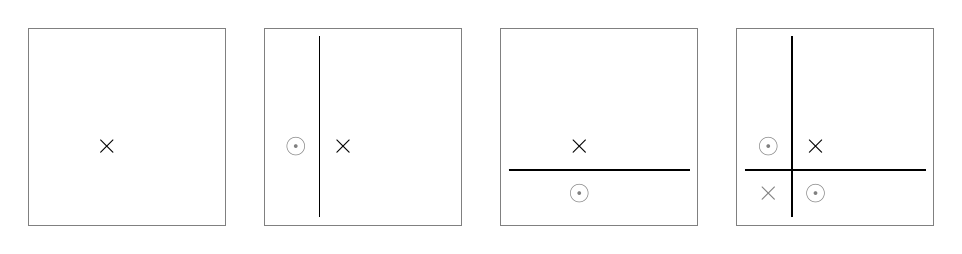
\begin{tikzpicture}
    \draw[gray] (0, 0) rectangle (2.5, 2.5);
    \node[black] at (1,1) {$\times$};

    \draw[gray] (3, 0) rectangle (5.5, 2.5); 
    \node[black] at (4,1) {$\times$};
    \draw[black] (3.7, 0.1) -- (3.7, 2.4); 
    \node[gray] at (3.4,1) {$\odot$};

    \draw[gray] (6, 0) rectangle (8.5, 2.5); 
    \node[black] at (7,1) {$\times$};
    \draw[black] (6.1, 0.7) -- (8.4, 0.7); 
    \node[gray] at (7,0.4) {$\odot$};

    \draw[gray] (9, 0) rectangle (11.5, 2.5); 
    \node[black] at (10,1) {$\times$};
    \draw[black] (9.1, 0.7) -- (11.4, 0.7); 
    \node[gray] at (10,0.4) {$\odot$};
    \draw[black] (9.7, 0.1) -- (9.7, 2.4); 
    \node[gray] at (9.4,1) {$\odot$};
    \node[gray] at (9.4,0.4) {$\times$};
  \end{tikzpicture}
  \caption{Examples of A-type cells (isolated wires with at most one $x$-plane and one $y$-plane).}
  \label{Fig:CellTypeA}
\end{figure}

\begin{figure}
  \centering
  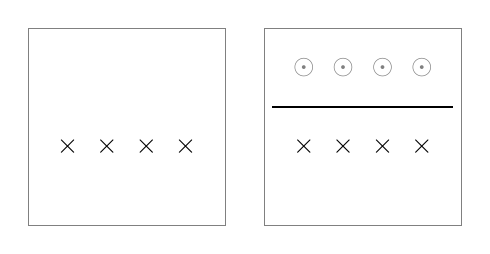
\begin{tikzpicture}
    \draw[gray] (0, 0) rectangle (2.5, 2.5);
    \node[black] at (0.5,1) {$\times$};
    \node[black] at (1.0,1) {$\times$};
    \node[black] at (1.5,1) {$\times$};
    \node[black] at (2.0,1) {$\times$};

    \draw[gray] (3, 0) rectangle (5.5, 2.5);
    \node[black] at (3.5,1) {$\times$};
    \node[black] at (4.0,1) {$\times$};
    \node[black] at (4.5,1) {$\times$};
    \node[black] at (5.0,1) {$\times$};
    \draw[black] (3.1, 1.5) -- (5.4, 1.5); 
    \node[gray] at (3.5,2) {$\odot$};
    \node[gray] at (4.0,2) {$\odot$};
    \node[gray] at (4.5,2) {$\odot$};
    \node[gray] at (5.0,2) {$\odot$};
  \end{tikzpicture}
  \caption{Examples of B1X-type cells ($x$-periodic array of wires with at most one $y$-plane).}
  \label{Fig:CellTypeB1}
\end{figure}

\begin{figure}
  \centering
  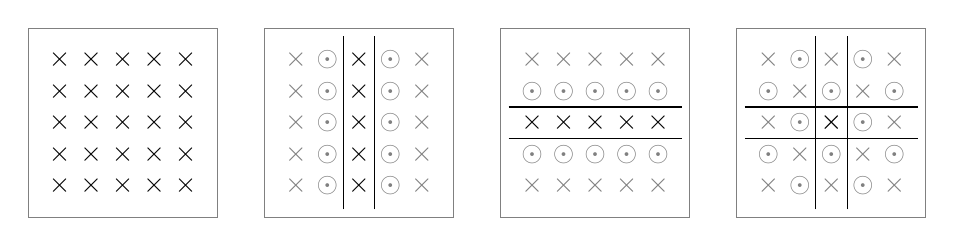
\begin{tikzpicture}
    \draw[gray] (0, 0) rectangle (2.4, 2.4);
    \foreach \x in {0.4,0.8,1.2,1.6,2.0}
    \foreach \y in {0.4,0.8,1.2,1.6,2.0}
      \node[black] at (\x,\y) {$\times$};

    \draw[gray] (3, 0) rectangle (5.4, 2.4);
    \foreach \y in {0.4,0.8,1.2,1.6,2.0}{
      \node[gray] at (3.4,\y) {$\times$};
      \node[gray] at (3.8,\y) {$\odot$};
      \node[black] at (4.2,\y) {$\times$};
      \node[gray] at (4.6,\y) {$\odot$};
      \node[gray] at (5.0,\y) {$\times$};
    }
    \draw[black] (4.0, 0.1) -- (4.0, 2.3);
    \draw[black] (4.4, 0.1) -- (4.4, 2.3);

    \draw[gray] (6, 0) rectangle (8.4, 2.4);
    \foreach \x in {6.4,6.8,7.2,7.6,8.0}{
      \node[gray] at (\x,0.4) {$\times$};
      \node[gray] at (\x,0.8) {$\odot$};
      \node[black] at (\x,1.2) {$\times$};
      \node[gray] at (\x,1.6) {$\odot$};
      \node[gray] at (\x,2.0) {$\times$};
    }
    \draw[black] (6.1, 1.0) -- (8.3, 1.0);
    \draw[black] (6.1, 1.4) -- (8.3, 1.4);

    \draw[gray] (9, 0) rectangle (11.4, 2.4);
    \foreach \x in {9.4, 10.2,11.0}{ 
    \foreach \y in {0.4, 1.2,2.0}
      \node[gray] at (\x,\y) {$\times$}; 
    \foreach \y in {0.8, 1.6}
      \node[gray] at (\x,\y) {$\odot$}; 
    }
    \foreach \x in {9.8, 10.6}{ 
    \foreach \y in {0.4, 1.2,2.0}
      \node[gray] at (\x,\y) {$\odot$}; 
    \foreach \y in {0.8, 1.6}
      \node[gray] at (\x,\y) {$\times$}; 
    }

    \node[black] at (10.2,1.2) {$\times$};

    \draw[black] (10.0, 0.1) -- (10.0, 2.3);
    \draw[black] (10.4, 0.1) -- (10.4, 2.3);
    \draw[black] (9.1, 1.4) -- (11.3, 1.4);
    \draw[black] (9.1, 1.0) -- (11.3, 1.0);
    \draw[black] (9.1, 1.4) -- (11.3, 1.4);
  \end{tikzpicture}
  \caption{Examples of C-type cells (doubly periodic arrays of wires).}
  \label{Fig:CellTypeC}
\end{figure}

\begin{figure}
  \centering
  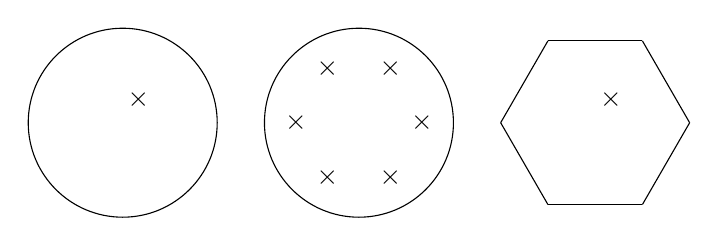
\begin{tikzpicture}
    \draw[black] (0, 0) circle[radius=1.2];
    \node[black] at (0.2,0.3) {$\times$};

    \draw[black] (3, 0) circle[radius=1.2];
    \foreach \phi in {0, 60, 120, 180, 240, 300}
      \node[black] at ({3+0.8*cos(\phi)},{0.8*sin(\phi)}) {$\times$};

    \foreach \phi in {0, 60, 120, 180, 240, 300}
      \draw[black] ({6+1.2*cos(\phi)},{1.2*sin(\phi)}) -- ({6+1.2*cos(\phi+60)},{1.2*sin(\phi+60)});
    \node[black] at (6.2,0.3) {$\times$};
  \end{tikzpicture}
  \caption{Examples of D-type cells. Left: isolated wire in a circular tube (D1). Middle: $\phi$-periodic ring of wires in a circular tube (D2). Right: wire in a polygon (D3).}
  \label{Fig:CellTypeD}
\end{figure}

Internally, cells are classified as belonging to one of these types:
\begin{description}
  \item[A]
  non-periodic cells with at most one \(x\) and one \(y\) plane
  \item[B1X]
  \(x\)-periodic cells without \(x\) planes and at most one \(y\) plane
  \item[B1Y]
  \(y\)-periodic cells without \(y\) planes and at most one \(x\) plane
  \item[B2X]
  cells with two \(x\) planes and at most one \(y\) plane
  \item[B2Y]
  cells with two \(y\) planes and at most one \(x\) plane
  \item[C1]
  doubly periodic cells without planes
  \item[C2X]
  doubly periodic cells with \(x\) planes
  \item[C2Y]
  doubly periodic cells with \(y\) planes
  \item[C3]
  doubly periodic cells with \(x\) and \(y\) planes
  \item[D1]
  round tubes without axial periodicity
  \item[D2]
  round tubes with axial periodicity
  \item[D3]
  polygonal tubes without axial periodicity
\end{description}

After the cell has been assembled and initialized, the cell type can be 
retrieved by the function
\begin{lstlisting}
std::string GetCellType();
\end{lstlisting}

\subsection{Dipole moments}
By default, \texttt{ComponentAnalyticField} uses the thin-wire approximation
for computing the electric field and potential. In this approach, 
dipole and higher-order terms are neglected which is usually a good   
approximation if the wire spacing is large compared to the diameter.
One can request dipole terms to be included in the calculation using
\begin{lstlisting}
void EnableDipoleTerms(const bool on = true);
\end{lstlisting}
Dipole terms are currently implemented only for cell types 
A, B1X, B1Y, B2X and B2Y.
To investigate whether dipole and higher order terms are significant, 
one can use the function
\begin{lstlisting}
bool MultipoleMoments(const unsigned int iw, const unsigned int order = 4,
                      const bool print = false, const bool plot = false, 
                      const double rmult = 1.,
                      const double eps = 1.e-4, const unsigned int nMaxIter = 20);
\end{lstlisting} 
\begin{description}
  \item[iw] index of the wire for which the multipole decomposition should be done,
  \item[order] order of the highest multipole moment to be taken into account,
  \item[print] flag to request verbose output during the minimisation step,
  \item[plot] flag to create a plot of the result of the multipole fit,
  \item[rmult] distance (in units of the wire radius) at which the potential 
               is to be calculated,
  \item[eps] ``small number'' used by the minimisation function to calculate the derivative matrix,
  \item[nMaxIter] max. number of iteration in the minimisation.
\end{description}

\subsection{Weighting fields}

By default, weighting fields and potentials will be calculated for 
all elements (wires, planes, \textit{etc.}) which were assigned a 
non-empty string as a label.

In addition to the weighting fields of 
the elements used for the calculation of the 
(actual) electric field, 
the weighting field for a strip segment of a plane 
can also be calculated. 
Strips can be defined using
\begin{lstlisting}
void AddStripOnPlaneX(const char direction, const double x,
                      const double smin, const double smax,
                      const std::string& label, const double gap = -1.);
void AddStripOnPlaneY(const char direction, const double y,
                      const double smin, const double smax,
                      const std::string& label, const double gap = -1.);
\end{lstlisting} 
\begin{description}
  \item[direction]
  orientation of the strip (\texttt{'y'} or \texttt{'z'} 
  in case of \(x\)-planes, \texttt{'x'} or \texttt{'z'} 
  in case of \(y\)-planes
  \item[x, y] coordinate of the plane on which the strip is located
  \item[smin, smax] min. and max. coordinate of the strip
\end{description}
The strip weighting field is calculated using an analytic expression for  
the field between two infinite parallel plates which are kept at 
ground potential except for the strip segment, which is raised to 1~V.
The anode-cathode distance \(d\) to be used for the evaluation of this 
expression can be set by the user (variable \texttt{gap} in 
\texttt{AddStripOnPlaneX}, \texttt{AddStripOnPlaneY}). 
If this variable is not specified (or set to a negative value), 
the following default values are used:
\begin{itemize}
  \item
  if two planes are present in the cell, \(d\) is  
  assumed to be the distance between those planes;
  \item
  if only one plane is present, \(d\) is taken to be 
  the distance to the nearest wire.
\end{itemize}

Similarly, pixels can be defined using
\begin{lstlisting}
void AddPixelOnPlaneX(const double x, const double ymin, const double ymax,
                      const double zmin, const double zmax,
                      const std::string& label, const double gap = -1., 
                      const double rot = 0.);
void AddPixelOnPlaneY(const double y, const double xmin, const double xmax,
                      const double zmin, const double zmax,
                      const std::string& label, const double gap = -1.,
                      const double rot = 0.);
\end{lstlisting}
The last (optional) parameter specifies the rotation angle (in rad) of the pixel in the plane.
Pixel weighting fields are calculated using the expressions given in 
Ref.~\cite{Riegler2014}.

When working in polar coordinates, strips and pixels are defined using
\begin{lstlisting}
void AddStripOnPlaneR(const char direction, const double r, const double smin    ,
                      const double smax, const std::string& label,
                      const double gap = -1.);
void AddStripOnPlanePhi(const char direction, const double phi, const double     smin,
                        const double smax, const std::string& label,
                        const double gap = -1.);
void AddPixelOnPlaneR(const double r,
                      const double phimin, const double phimax,
                      const double zmin, const double zmax,
                      const std::string& label, const double gap = -1.);
void AddPixelOnPlanePhi(const double phi,
                        const double rmin, const double rmax,
                        const double zmin, const double zmax,
                        const std::string& label, const double gap = -1.);
\end{lstlisting} 
Valid strip directions are \texttt{'p'} ($\phi$) or \texttt{'z'} for 
circular planes and \texttt{'r'} or \texttt{'z'} for $\phi$ planes.

In periodic chambers, the electric field is identical in all copies of the 
basic cell, but the weighting fields of the wires of one copy are as a rule 
not the same as the weighting fields of the wires of another copy.
\texttt{ComponentAnalyticField} will, by default, compute the 
weighting fields and potentials by considering only the basic cell -- 
suppressing all periodicities. This is a good approximation if the wires 
being read out are surrounded by many other wires in the basic cell.

This behaviour can be controlled using the function
\begin{lstlisting}
void SetNumberOfCellCopies(const unsigned int nfourier);
\end{lstlisting}
The argument (\texttt{nfourier}) must be 0 or an integral power of 2.

If the argument is 0,
the weighting field and potential will be computed using the same 
functions that are used for the electric field, \textit{i. e.} they 
will exhibit the same periodicity. 
This should be used if one is interested only in the signals induced in 
the planes (and not in the wire signals) or 
if all copies of the read-out wires are interconnected. 

If the argument is non-zero, \texttt{SetNumberOfCellCopies} 
sets the number of copies of the basic cell to be included in the 
weighting field calculation. 
Requesting a large number of copies is meaningful only in chambers 
which contain equipotential planes - convergence is poor otherwise.

\subsection{Wire displacements}
The forces acting on a wire and the wire displacement that results from 
these forces can be computed using the methods
\begin{lstlisting}
bool ForcesOnWire(const unsigned int iw, 
                  std::vector<double>& xMap, std::vector<double>& yMap,
                  std::vector<std::vector<double> >& fxMap,
                  std::vector<std::vector<double> >& fyMap);
\end{lstlisting}
and
\begin{lstlisting}
bool WireDisplacement(const unsigned int iw, const bool detailed,
                      std::vector<double>& csag, std::vector<double>& xsag,
                      std::vector<double>& ysag, double& stretch,
                      const bool print = true);
\end{lstlisting}
of \texttt{ComponentAnalyticField}. In both methods, the argument 
\texttt{iw} is the index of the wire (you can use the function \texttt{PrintCell} to print a list of all wires in the cell layout).
By default, both gravitational force and electrostatic force are 
taken into account for computing the displacement. 
This can be changed using
\begin{lstlisting}
void EnableGravity(const bool on = true);
void EnableElectrostaticForce(const bool on = true);
\end{lstlisting}
The direction in which gravity acts on the wires can be set using
\begin{lstlisting}
void SetGravity(const double dx, const double dy, const double dz);
\end{lstlisting}
The three arguments are the components of a vector indicating the 
direction in which gravity pulls on the wires. 
Only the direction of the vector is used, not its normalisation. 

The function \texttt{WireDisplacement} fills the vector 
\texttt{csag} with a set of coordinates along the wire and 
the vectors \texttt{xsag}, \texttt{ysag} with the $x$ and $y$ components 
of the sag profile at these coordinates, and sets the variable 
\texttt{stretch} to the relative elongation.  
It offers two levels of accuracy.
\begin{itemize}
\item
With the flag \texttt{detailed} set to \texttt{false}, only the force 
acting on the wire in its nominal position is used to compute the sag.
The wire sag that results from such a force is parabolic, since it 
results from an elastic elongation. The shape is not a hyperbolic cosine, 
this would be the case of a freely hanging wire.
This approach is incorrect if the wire is nominally in an almost stable 
position while there are substantial forces acting on the wire in 
neighbouring positions.
\item
If the flag \texttt{detailed} is set to \texttt{true}, the method also 
considers the force acting on the wire in the vicinity of its nominal 
position.
The electrostatic forces are computed by solving the capacitance equations for a set of wire locations on a regular grid around the nominal location 
and interpolating the resulting table of forces.
The number of grid lines can be set using
\begin{lstlisting}
void SetScanningGrid(const unsigned int nX, const unsigned int nY);
\end{lstlisting}
The default is 11 lines in both $x$ and $y$.
By default, the range of wire shifts for which the forces are computed, 
is selected automatically by enlarging by a scaling factor 
(default: 2) the zeroth order 
estimates of the shift, and restricting this to the largest area around 
the wire which is free of other cell elements. 
The scaling factor can be set using 
\begin{lstlisting}
void SetScanningAreaFirstOrder(const double scale = 2.);
\end{lstlisting}
If the wire movements are expected to be very large, then one may wish 
to set the scanning area to the largest area around the wire which is 
free from other cell elements:
\begin{lstlisting}
void SetScanningAreaLargest();
\end{lstlisting}
You may also manually set the scanning area by specifying a lower $x$, 
an upper $x$, a lower $y$  and an upper $y$ which together describe a 
rectangular area relative to the nominal position of the wire 
under consideration.
\begin{lstlisting}
void SetScanningArea(const double xmin, const double xmax, 
                     const double ymin, const double ymax);
\end{lstlisting}
By default, the calculation stops if a point of the wire is found at a 
position not covered by the scanning area, whether set manually or 
automatically.
If you enable extrapolation using
\begin{lstlisting}
void EnableExtrapolation(const bool on = true);
\end{lstlisting}
then the force on the wire at such a point will be computed by 
extrapolating the force table.
It is usually a better strategy to pick a scanning area that covers all 
wire positions -- if this is not possible, then the wire is probably not 
in a stable position (\textit{i.e.} it will move against other electrodes).
\end{itemize}
In the detailed approach, the differential equation that governs the wire 
sag is numerically solved using a multiple shooting method in which each 
shot is traced with a Runge-Kutta-Nystroem method, and in which the 
boundary and matching conditions are minimised with a Newton method with 
Broyden rank-1 updates of the derivative matrix.
The number of shots and the number of integration steps within each shot 
can be set by the user
\begin{lstlisting}
void SetNumberOfShots(const unsigned int n);
void SetNumberOfSteps(const unsigned int n);
\end{lstlisting}

The function \texttt{ForcesOnWire} fills the vectors \texttt{xMap}, 
\texttt{yMap} with the coordinates of the scanning grid lines 
(relative to the nominal wire position) and the vectors \texttt{fxMap},  
\texttt{fyMap} with the $x$ and $y$ components of the electrostatic 
force at the grid points. 
The scanning grid can be set using the same methods as 
for \texttt{WireDisplacement}. 

\subsection{Optimisation}
\texttt{ComponentAnalyticField} includes a set of methods that 
vary the potentials of a set of electrodes in an attempt to match as 
closely as possible a function of the potential and field 
(field function) to a given target value. 
\begin{itemize}
\item
The method 
\begin{lstlisting}
bool OptimiseOnTrack(const std::vector<std::string>& groups,
    const std::string& field_function, const double target,
    const double x0, const double y0, const double x1, const double y1,
    const unsigned int nP = 20, const bool print = true);
\end{lstlisting}
compares target and field function on \texttt{nP} sampling points 
along a straight line between $\left(x_{0}, y_{0}\right)$ and 
$\left(x_{1}, y_{1}\right)$.
This function can be used \textit{e. g.} to adjust the potentials on a 
drift electrode in a TPC to get the proper drift field.
\item 
\begin{lstlisting}
bool OptimiseOnGrid(const std::vector<std::string>& groups,
    const std::string& field_function, const double target,
    const double x0, const double y0, const double x1, const double y1,
    const unsigned int nX = 10, const unsigned int nY = 10,
    const bool print = true);
\end{lstlisting}
compares target and field function on a regular $x-y$ (or $r-\phi$) grid.
The extent of the grid area is defined by the two corners 
$\left(x_{0}, y_{0}\right), \left(x_{1}, y_{1}\right)$ and the grid 
density is defined by \texttt{nX}, \texttt{nY} 
(number of lines in $x$ and $y$).
\item
\begin{lstlisting}
bool OptimiseOnWires(const std::vector<std::string>& groups,
    const std::string& field_function, const double target,
    const std::vector<unsigned int>& wires, const bool print = true);
\end{lstlisting}
compares target and field function on the surfaces of a set of wires 
(the vector \texttt{wires} contains the wire indices).
This function can be used \textit{e. g.} to adjust the voltages on the  
anode wires such that the field in their proximity has a given value. 
\end{itemize}
The vector \texttt{groups} contains the labels of the electrodes 
for which to adjust the potentials.
Electrodes that are put together in a group are shifted collectively.
In the expression \texttt{field\_function} the following variables may be 
used:
\begin{itemize}
  \item
  \texttt{x} or \texttt{r} ($x$ or $r$ coordinate),
  \item
  \texttt{y} or \texttt{phi} ($y$ or $\phi$ coordinate),
  \item
  \texttt{ex} or \texttt{er} ($x$ or $r$-component of the electric field),
  \item
  \texttt{ey} or \texttt{ephi} ($y$ or $\phi$-component of the electric field),
  \item
  \texttt{e} (norm of the electric field),
  \item
  \texttt{v} (electric potential). 
\end{itemize} 
More variables can be added on demand.

If the flag \texttt{print} is set to \texttt{true}, 
some optimisation information is printed at each cycle.

The method used is that of repeated Householder steps minimising 
(in the Euclidean norm) the difference between target and field 
function. Several conditions can cause the iteration to be stopped:
\begin{itemize}
\item
the user defined maximum number of iterations is reached,
\item
the relative change in Euclidean distance between the target and field 
function (on the sampling points) drops below threshold $\varepsilon$, 
\item
the maximum distance (of all sampling points) between target and field 
function becomes smaller than a threshold distance.
\end{itemize}
These parameters can be set using the method
\begin{lstlisting} 
void SetOptimisationParameters(const double dist = 1.,
                               const double eps = 1.e-4,
                               const unsigned int nMaxIter = 10);
\end{lstlisting}
The parameter $\varepsilon$ is also used for computing the numerical 
derivatives needed for the covariance matrix. A larger value (say 1) 
should be chosen when you know you are far from the optimised value 
and a smaller value (say $10^{-4}$) when your initial guess is quite good.

\section{neBEM}
The nearly exact Boundary Element Method (neBEM) solver discretizes
the boundary of the domain in triangular and rectangular elements 
and computes the surface charge density on each of these elements that is
required to satisfy the applied boundary conditions. 
Once the charge density distribution has been obtained, 
the potential and field can be evaluated at any point in the domain. 
A detailed description of the technique can be found in 
Refs.~\cite{Mukhopadhyay2006Eng,Mukhopadhyay2006,Mukhopadhyay2009}. 
 
The \texttt{ComponentNeBem3d} interface class requires as input a 
\texttt{GeometrySimple} object with its list of solids and associated 
media. 
\begin{lstlisting}
void ComponentNeBem3d::SetGeometry(Geometry* geo);
\end{lstlisting}
The boundary conditions to be applied to each solid can be set using
\begin{lstlisting}
void Solid::SetBoundaryPotential(const double v);
\end{lstlisting}
in case of a conductor at fixed potential (Dirichlet boundary conditions) 
or 
\begin{lstlisting}
void Solid::SetBoundaryDielectric();
\end{lstlisting}
in case of a dielectric-dielectric interface. 
In the latter case (Neumann boundary conditions), 
the normal component of the displacement field $\mathbf{D} = \varepsilon\mathbf{E}$ is required to be continuous at the boundary of the solid,
\begin{equation*}
  \mathbf{n}\cdot\left(\varepsilon^{+}\mathbf{E}^{+} - \varepsilon^{-}\mathbf{E}^{-}\right).
\end{equation*}

During initialisation, \texttt{ComponentNeBem3d}
\begin{itemize}
\item
retrieves the surface panels from the \texttt{Solid} objects 
present in the geometry,
\item
searches for and eliminates overlaps between the panels,  
\item
and splits the resulting polygons into rectangular and triangular ``primitives''.
\end{itemize}
These ``primitives'' are then passed on to neBEM, where they are further 
subdivided into ``elements'' (rectangles and right-angled triangles).
A special case are \texttt{SolidWire} objects which are represented 
as one-dimensional straight line primitives and elements 
(corresponding to the thin-wire approximation used also 
in \texttt{ComponentAnalyticField}). 
The elements should be small enough such that the distribution of the 
charge density on them be approximated as uniform.
The size of the elements can be controlled using the functions
\begin{lstlisting}
void SetTargetElementSize(const double length);
void SetMinMaxNumberOfElements(const unsigned int nmin, const unsigned int nmax);
\end{lstlisting}
\begin{description}
\item[length] preferred linear size of the elements, measured along their edges.
\item[nmin,nmax] smallest and largest number of elements produced along either axis of a single primitive.
\end{description}
One can also request different target element sizes for each 
\texttt{Solid} object, using
\begin{lstlisting}
void Solid::SetDiscretisationLevel(const double dis);
\end{lstlisting} 

After splitting the primitives into elements, 
neBEM determines the influence matrix $K$ and 
the right-hand side vector\footnote{In a system with only Dirichlet 
boundary conditions, the right-hand side vector is given by the 
potentials at the elements, $b_{i} = V_{i}$.}
of the system of equations
\begin{equation*}
K \boldsymbol{\rho} = \mathbf{b},
\end{equation*}
inverts the matrix and computes the surface charge density $\rho_{i}$ 
of every element,
\begin{equation*}
\rho_{i} = K^{-1}_{ij} b_{j}. 
\end{equation*}

\subsection{Weighting fields}
If a \texttt{Solid} object has been given a label using 
\begin{lstlisting}
void Solid::SetLabel(const std::string& label);
\end{lstlisting}
neBEM will compute its weighting field at the same time as 
the electric field.
One can assign the same label to multiple \texttt{Solid} objects.
The weighting field corresponding to this label will then be 
computed by setting the potential of all elements associated to solids 
with this label to 1\,V (and grounding all other conducting elements).

\section{Parameterisations}
The class \texttt{ComponentUser} takes the electric field and potential
from a user-defined function.
\begin{lstlisting}
void SetElectricField(std::function<void(const double, const double, const double, 
                                         double& double&, double&)> f);
void SetPotential(std::function<double(const double, const double, const double)> f);
\end{lstlisting}
\begin{description}
  \item[f] user function
\end{description}
The signature of the electric field function is \texttt{void(const double, const double, const double, double\&, double\&, double\&)}, 
the first three arguments being the coordinates $x, y, z$ and the 
last three (reference) arguments being the components of the electric 
field (to be assigned in the function).
The potential function takes the coordinates $x, y, z$ as arguments and
returns the potential. 
Similar functions are available to set the weighting field and potential,
and the magnetic field.

Alternatively, \texttt{ComponentUser} also allows one to define the 
electric field and potential in string expressions, which are then
just-in-time compiled internally using the ROOT C++ interpreter.
\begin{lstlisting}
void SetElectricField(const std::string& expression);
void SetPotential(const std::string& expression);
\end{lstlisting}
\begin{description}
  \item[expression] a compileable C++ expression.
\end{description}
Valid parameter names are \texttt{x}, \texttt{y}, \texttt{z}. 
The expression used for evaluating the electric field 
shall assign the variables \texttt{ex}, \texttt{ey}, \texttt{ez} 
(corresponding to the three field components). 
If a field component is not assigned in the expression, it is assumed 
to be zero.

As an example, let us consider the electric field in the bulk 
of an overdepleted planar silicon sensor, given by
\begin{equation*}
E\left(x\right) = \frac{V - V_{\text{dep}}}{d} + 
                    2x \frac{V_{\text{dep}}}{d^{2}},
\end{equation*}
where \(V\) is the applied bias voltage, \(V_{\text{dep}}\) is 
the depletion voltage, and \(d\) is the thickness of the diode.
\begin{lstlisting}
MediumSilicon si;
// Detector thickness
const double d = 0.1;

ComponentUser cmp;
cmp.SetArea(0., -2 * d, -2 * d, d, 2 * d, 2 * d);
cmp.SetMedium(&si);
auto efield = [](const double x, const double y, const double z,
                 double& ex, double& ey, double& ez) { 

  // Depletion voltage
  const double vdep = 160.;
  // Applied voltage
  const double v = 200.;

  ey = ez = 0.;
  ex = (v - vdep) / d + 2 * x * vdep / (d * d);
};
cmp.SetElectricField(efield);
\end{lstlisting}

Using the JIT-compilation approach, the above example would look like this.
\begin{lstlisting}
MediumSilicon si;
// Detector thickness
const double d = 0.1;

ComponentUser cmp;
cmp.SetArea(0., -2 * d, -2 * d, d, 2 * d, 2 * d);
cmp.SetMedium(&si);
// Depletion voltage
const double vdep = 160.;
// Applied voltage
const double v = 200.;

std::string efield = "ex = " + std::to_string((v - vdep) / d) + 
                     "2 * x * " + std::to_string(vdep / (d * d));
cmp.SetElectricField(efield);
\end{lstlisting}

\section{Other components}
For simple calculations, the class \texttt{ComponentConstant} can be used. 
As the name implies, it provides a uniform electric field. 
The electric field and potential can be specified using
\begin{lstlisting}
void SetElectricField(const double ex, const double ey, const double ez);
void SetPotential(const double x, const double p, const double z, const double v);
\end{lstlisting}
\begin{description}
  \item[ex, ey, ez]
  components of the electric field
  \item[x, y, z]
  coordinates where the potential is specified
  \item[v]
  voltage at the given position
\end{description}
The weighting field and potential can be set using
\begin{lstlisting}
void SetWeightingField(const double wx, const double wy, const double wz,
                       const std::string label);
void SetWeightingPotential(const double x, const double y, const double z,
                           const double v);
\end{lstlisting}
\begin{description}
  \item[wx,wy,wz] components of the weighting field
  \item[label] identifier of the weighting field/electrode
  \item[x, y, z] coordinates where the weighting potential is specified
  \item[v] weighting potential at the given position 
\end{description}

\section{Visualizing the field}

The class \texttt{ViewField} provides some basic functions 
for plotting the potential and field of a component/sensor.

The \texttt{Component} or \texttt{Sensor} from which to retrieve the 
field/potential to be plotted is set by means of
\begin{lstlisting}
void SetComponent(Component* c);
void SetSensor(Sensor* s);
\end{lstlisting}

By default, the voltage range is retrieved from the 
minimum and maximum values of the 
potential in the component/sensor, and
the range of the electric and weighting fields is
``guessed'' by taking random samples.
This feature can be switched on or off using the function
\begin{lstlisting}
void EnableAutoRange(const bool on = true, const bool samplePotential = true);
\end{lstlisting}
The flag \texttt{samplePotential} indicates whether the range of the 
potential should be determined by random sampling or if \texttt{ViewField}
should first try to retrieve it from the component/sensor. 

If the ``auto-range'' feature is disabled,
the range of the function to be plotted needs to be set using
\begin{lstlisting}
void SetVoltageRange(const double vmin, const double vmax);
void SetElectricFieldRange(const double emin, const double emax);
void SetWeightingFieldRange(const double wmin, const double wmax);
\end{lstlisting}

\subsection{One-dimensional plots}
The function 
\begin{lstlisting}
void PlotProfile(const double x0, const double y0, const double z0,
                 const double x1, const double y1, const double z1,
                 const std::string& option = "v",
                 const bool normalised = true);
\end{lstlisting}
plots the potential or field (depending on the parameter \texttt{option}) 
along the line  
\(\left(x_{0}, y_{0}, z_{0}\right) \rightarrow 
  \left(x_{1}, y_{1}, z_{1}\right)\).
With the flag \texttt{normalised} set to \texttt{true} (default), 
normalised coordinates $\left[0, 1\right]$ are used for the $x$-axis. 

Similar functions are available for visualizing weighting potentials and fields.
\begin{lstlisting}
void PlotContourWeightingField(const std::string& label, const std::string& option);
void PlotWeightingField(const std::string& label, const std::string& option,
                        const std::string& drawopt);
void PlotProfileWeightingField(const std::string& label,
                   const double x0, const double y0, const double z0,
                   const double x1, const double y1, const double z1,
                   const std::string& option = "v",
                   const bool normalised = true);
\end{lstlisting}
\begin{description}
  \item[label] identifier of the electrode for which to plot the weighting field/potential.
\end{description}

\subsection{Two-dimensional plots}

The functions 
\begin{lstlisting}
void PlotContour(const std::string& option = "v");
void Plot(const std::string& option = "v", const std::string& drawopt = "");
\end{lstlisting}
create a contour plot or another two-dimensional plot in the chosen viewing plane.
The quantity to be plotted is set using the parameter \texttt{option} 
(see Table~\ref{Tab:ViewFieldOptionStrings}).
\begin{table}
  \centering
  \caption{\texttt{ViewField} option strings and corresponding quantities.}
  \label{Tab:ViewFieldOptionStrings}
  \begin{tabular}{l l} 
    \toprule
    Quantity & \texttt{option} \\
    \midrule
    Electrostatic potential & \texttt{"v"}, \texttt{"p"}, \texttt{"phi"} \\
    Magnitude of the electric field ($\left|\mathbf{E}\right|$) & \texttt{"e"}, \texttt{"emag"}, \texttt{"norm"} \\
    $x$-component of the electric field ($E_{x}$) & \texttt{"ex"} \\ 
    $y$-component of the electric field ($E_{y}$) & \texttt{"ey"} \\ 
    $z$-component of the electric field ($E_{z}$) & \texttt{"ez"} \\
    \midrule 
    Magnitude of the magnetic field ($\left|\mathbf{B}\right|$) & \texttt{"bmag"} \\
    $x$-component of the magnetic field ($B_{x}$) & \texttt{"bx"} \\ 
    $y$-component of the magnetic field ($B_{y}$) & \texttt{"by"} \\ 
    $z$-component of the magnetic field ($B_{z}$) & \texttt{"bz"} \\ 
    \bottomrule
  \end{tabular}
\end{table}
The parameter \texttt{drawopt} is passed on to the function \texttt{Draw()} of the
ROOT \texttt{TF2} class and sets the plotting options. For instance,
\begin{lstlisting}
ViewField view;
view.Plot("v", "SURF4");
\end{lstlisting}
will create a surface plot of the potential.

The viewing plane and the region to be drawn 
can be specified using
\begin{lstlisting}
void SetArea(const double xmin, const double ymin, const double xmax, const double ymax);
void SetPlane(const double fx, const double fy, const double fz,
              const double x0, const double y0, const double z0);
void Rotate(const double angle);
\end{lstlisting}
\begin{description}
  \item[xmin, ymin, xmax, ymax] plot range in ``local coordinates'' (in the current viewing plane).
  \item[fx, fy, fz] normal vector of the plane.
  \item[x0, y0, z0] in-plane point.
  \item[angle] rotation angle (in radian).
\end{description}
By default, the viewing plane is the $x-y$ plane (at $z = 0$) and the 
plot range is retrieved from the bounding box of the component/sensor.
The default viewing plane can be restored using 
\begin{lstlisting}
void SetPlaneXY();
\end{lstlisting}
and the feature to determine the plot area from the bounding box can be activated using 
\begin{lstlisting}
void SetArea();
\end{lstlisting}
 
The density of the plotting grid can be set using
\begin{lstlisting}
void SetNumberOfSamples1d(const unsigned int n);
void SetNumberOfSamples2d(const unsigned int nx, const unsigned int ny);
\end{lstlisting}
\begin{description}
  \item[n, nx, ny]
  number of points in \(x\) and \(y\) direction 
  (default for one-dimensional plots: \(n = 1000\);
   default for two-dimensional plots: \(n_{x} = n_{y} = 200\)) 
\end{description}

The number of contour levels can be set using
\begin{lstlisting}
void SetNumberOfContours(const unsigned int n);
\end{lstlisting}

\subsection{Field lines}
The function
\begin{lstlisting}
void PlotFieldLines(const std::vector<double>& x0,
                    const std::vector<double>& y0,
                    const std::vector<double>& z0,
                    const bool electron = true, const bool axis = true,
                    const short col = kOrange - 3)
\end{lstlisting}
computes and draws electric field lines from a set of starting points, 
given by the vectors \texttt{x0}, \texttt{y0}, \texttt{z0}. 
The flag \texttt{electron} specifies whether the field lines should 
be calculated for a negative (electron-like) test charge 
or for a positive test charge.

A useful helper function for determining the starting points is
\begin{lstlisting}
bool EqualFluxIntervals(const double x0, const double y0, const double z0,
                        const double x1, const double y1, const double z1,
                        std::vector<double>& xf, std::vector<double>& yf,
                        std::vector<double>& zf,
                        const unsigned int nPoints = 20) const;
\end{lstlisting} 
which fills the vectors \texttt{xf}, \texttt{yf}, \texttt{zf} with 
the coordinates of \texttt{nPoints} along the line 
$\left(x_{0}, y_{0}, z_{0}\right) -- \left(x_{1}, y_{1}, z_{1}\right)$ 
which are spaced by equal flux intervals.
The flux is computed by integrating the electric field component 
that is in the viewing plane and perpendicular to the line.

If the flux changes sign over the track, then points are only generated 
over the parts of the line where the flux is positive if the total flux 
over the line is positive. 
Conversely, if the total flux is negative, points are generated only in 
areas where the flux is negative. 

A similar function is
\begin{lstlisting}
bool FixedFluxIntervals(const double x0, const double y0, const double z0,
                        const double x1, const double y1, const double z1,
                        std::vector<double>& xf, std::vector<double>& yf,
                        std::vector<double>& zf,
                        const double interval = 10.) const;
\end{lstlisting}
It fills the vectors \texttt{xf}, \texttt{yf}, \texttt{zf} with 
the coordinates of points that are spaced by a given flux interval 
(in units of V).

\section{Inspecting the field}
The \texttt{Component} base class provides functions for inspecting the 
field, in particular for determining the electric flux over a surface.
\begin{lstlisting}
double IntegrateFluxSphere(const double xc, const double yc, const double zc,
                           const double r, const unsigned int nI = 20);
\end{lstlisting}
calculates the charge (in fC) enclosed in a sphere of radius $r$ centred at 
$\left(x_{c}, y_{c}, z_{c}\right)$ using Gauss's law, \ie by 
integrating the normal component of the electric field over the 
surface of the sphere, 
\begin{equation*}
  Q = \varepsilon_{0} \oint \mathbf{E}\cdot \text{d}\mathbf{A}.
\end{equation*}  
Similarly,
\begin{lstlisting}
double IntegrateFluxCircle(const double xc, const double yc, 
                           const double r, const unsigned int nI = 50);
\end{lstlisting}
calculates the line charge (in fC\,/\,cm) contained in a circle of radius $r$ 
centred at $\left(x_{c}, y_{c}\right)$.  
The integrations are performed using six-point Gaussian quadrature. 
The number of integration intervals can be set as a parameter. 

The integral of the flux over a parallelogram can be calculated using 
the function
\begin{lstlisting}
double IntegrateFluxParallelogram(const double x0, const double y0, const double z0,
                                  const double dx1, const double dy1, const double dz1,
                                  const double dx2, const double dy2, const double dz2,
                                  const unsigned int nU = 20, const unsigned int nV = 20); 
\end{lstlisting}
\begin{description}
  \item[x0,y0,z0] coordinates of one of the corners of the parallelogram,
  \item[dx1,dy1,dz1] direction vector from $\left(x_{0}, y_{0}, z_{0}\right)$ 
                     to one of the adjacent corners,
  \item[dx2,dy2,dz2] direction vector to the other adjacent corner,
  \item[nU,nV] number of integration intervals along the two directions.
\end{description}
The result is given in units of V\,cm.
\section{Sensor}

The \texttt{Sensor} class can be viewed as a composite of components. 
In order to obtain a complete description of a detector, 
it is sometimes useful to combine fields from different 
\texttt{Component} objects.
For instance, one might wish to use a field map for the electric field, 
calculate the weighting field using analytic methods, 
and use a parameterized \(B\) field. 
Superpositions of several electric, magnetic and weighting fields are also possible. 


Components are added using
\begin{lstlisting}
void AddComponent(Component* comp);
void AddElectrode(Component* comp, std::string label);
\end{lstlisting}
While \texttt{AddComponent} tells the \texttt{Sensor} that the 
respective \texttt{Component} should be included in the calculation 
of the electric and magnetic field, 
\texttt{AddElectrode} requests the weighting field named \texttt{label} 
to be used for computing the corresponding signal.

To deactivate (or activate) a component after having added it, the 
function
\begin{lstlisting}
void EnableComponent(const unsigned int i, const bool on);
\end{lstlisting}
can be used. Components that have been deactivated are not taken into 
account when calculating the electric field but are not removed from the list.
Similarly, 
\begin{lstlisting}
void EnableMagneticField(const unsigned int i, const bool on);
\end{lstlisting}
can be used to deactivate (or activate) the magnetic field of a 
given component. 

To reset the sensor, thereby removing all components and electrodes, use
\begin{lstlisting}
void Clear();
\end{lstlisting}

The total electric and magnetic fields 
(sum over all components) at a given position are accessible through 
the functions \texttt{ElectricField} and \texttt{MagneticField}.
The syntax is the same as for the corresponding functions of the 
\texttt{Component} classes.
Unlike the fields, materials cannot overlap. 
The function \texttt{Sensor::GetMedium}, therefore, 
returns the first valid drift medium found. 
 
The \texttt{Sensor} acts as an interface to the transport classes.

For reasons of efficiency, it is sometimes useful to restrict 
charge transport, ionization and similar calculations to a 
certain region of the detector.
This ``user area'' can be set by
\begin{lstlisting}
void SetArea(const double xmin, const double ymin, const double zmin,
             const double xmax, const double ymax, const double zmax);
\end{lstlisting} 
\begin{description}
\item[xmin, \dots, zmax]
corners of the bounding box within which transport is enabled. 
\end{description}
Calling \texttt{SetArea()} (without arguments) sets the 
user area to the envelope of all components (if such an envelope exists).

In addition, the \texttt{Sensor} class takes care of 
signal calculations (Chapter~\ref{Chap:Signals}).

